%% Преамбула TeX-файла

% 1. Стиль и язык
\documentclass[utf8x, 14pt]{G7-32} % Стиль (по умолчанию будет 14pt)

% Остальные стандартные настройки убраны в preamble.inc.tex.
\sloppy

% Настройки стиля ГОСТ 7-32
% Для начала определяем, хотим мы или нет, чтобы рисунки и таблицы нумеровались в пределах раздела, или нам нужна сквозная нумерация.
\EqInChapter % формулы будут нумероваться в пределах раздела
\TableInChapter % таблицы будут нумероваться в пределах раздела
\PicInChapter % рисунки будут нумероваться в пределах раздела

% Добавляем гипертекстовое оглавление в PDF
\usepackage[
bookmarks=true, colorlinks=true, unicode=true,
urlcolor=black,linkcolor=black, anchorcolor=black,
citecolor=black, menucolor=black, filecolor=black,
]{hyperref}
\usepackage{pgfplots}
\usepackage{nomencl}

\usepackage{float}


\AfterHyperrefFix

\usepackage{microtype}% полезный пакет для микротипографии, увы под xelatex мало чего умеет, но под pdflatex хорошо улучшает читаемость
\usepackage{indentfirst}

% Тире могут быть невидимы в Adobe Reader
\ifInvisibleDashes
\MakeDashesBold
\fi

\usepackage{graphicx}   % Пакет для включения рисунков

% С такими полями оно работает по-умолчанию:
% \RequirePackage[left=20mm,right=10mm,top=20mm,bottom=20mm,headsep=0pt,includefoot]{geometry}
% Если вас тошнит от поля в 10мм --- увеличивайте до 20-ти, ну и про переплёт не забывайте:
\geometry{right=10mm}
\geometry{left=30mm}
\geometry{bottom=20mm}
\geometry{ignorefoot}% считать от нижней границы текста


% Пакет Tikz
\usepackage{tikz}
\usetikzlibrary{arrows,positioning,shadows}

% Произвольная нумерация списков.
\usepackage{enumerate}

% ячейки в несколько строчек
\usepackage{multirow}

% itemize внутри tabular
\usepackage{paralist,array}

%\setlength{\parskip}{1ex plus0.5ex minus0.5ex} % разрыв между абзацами
\setlength{\parskip}{1ex} % разрыв между абзацами
\usepackage{blindtext}

% Центрирование подписей к плавающим окружениям
%\usepackage[justification=centering]{caption}

\usepackage{newfloat}
\DeclareFloatingEnvironment[
placement={!ht},
name=Equation
]{eqndescNoIndent}
\edef\fixEqndesc{\noexpand\setlength{\noexpand\parindent}{\the\parindent}\noexpand\setlength{\noexpand\parskip}{\the\parskip}}
\newenvironment{eqndesc}[1][!ht]{%
    \begin{eqndescNoIndent}[#1]%
\fixEqndesc%
}
{\end{eqndescNoIndent}}

\usepackage{afterpage}

\newcommand\blankpage{
	\null
	\thispagestyle{empty}
	\newpage
}



% Настройки листингов.
\ifPDFTeX
% 8 Листинги

\usepackage{listings}

% Значения по умолчанию
\lstset{
  basicstyle= \footnotesize,
  breakatwhitespace=true,% разрыв строк только на whitespacce
  breaklines=true,       % переносить длинные строки
%   captionpos=b,          % подписи снизу -- вроде не надо
  inputencoding=koi8-r,
  numbers=left,          % нумерация слева
  numberstyle=\footnotesize,
  showspaces=false,      % показывать пробелы подчеркиваниями -- идиотизм 70-х годов
  showstringspaces=false,
  showtabs=false,        % и табы тоже
  stepnumber=1,
  tabsize=4,              % кому нужны табы по 8 символов?
  frame=single,
  xleftmargin=2.4em,
  framexleftmargin=2em
}

% Стиль для псевдокода: строчки обычно короткие, поэтому размер шрифта побольше
\lstdefinestyle{pseudocode}{
  basicstyle=\small,
  keywordstyle=\color{black}\bfseries\underbar,
  language=Pseudocode,
  numberstyle=\footnotesize,
  commentstyle=\footnotesize\it
}

% Стиль для обычного кода: маленький шрифт
\lstdefinestyle{realcode}{
  basicstyle=\scriptsize,
  numberstyle=\footnotesize
}

% Стиль для коротких кусков обычного кода: средний шрифт
\lstdefinestyle{simplecode}{
  basicstyle=\footnotesize,
  numberstyle=\footnotesize
}

% Стиль для BNF
\lstdefinestyle{grammar}{
  basicstyle=\footnotesize,
  numberstyle=\footnotesize,
  stringstyle=\bfseries\ttfamily,
  language=BNF
}

% Определим свой язык для написания псевдокодов на основе Python
\lstdefinelanguage[]{Pseudocode}[]{Python}{
  morekeywords={each,empty,wait,do},% ключевые слова добавлять сюда
  morecomment=[s]{\{}{\}},% комменты {а-ля Pascal} смотрятся нагляднее
  literate=% а сюда добавлять операторы, которые хотите отображать как мат. символы
    {->}{\ensuremath{$\rightarrow$}~}2%
    {<-}{\ensuremath{$\leftarrow$}~}2%
    {:=}{\ensuremath{$\leftarrow$}~}2%
    {<--}{\ensuremath{$\Longleftarrow$}~}2%
}[keywords,comments]

% Свой язык для задания грамматик в BNF
\lstdefinelanguage[]{BNF}[]{}{
  morekeywords={},
  morecomment=[s]{@}{@},
  morestring=[b]",%
  literate=%
    {->}{\ensuremath{$\rightarrow$}~}2%
    {*}{\ensuremath{$^*$}~}2%
    {+}{\ensuremath{$^+$}~}2%
    {|}{\ensuremath{$|$}~}2%
}[keywords,comments,strings]

% Подписи к листингам на русском языке.
\renewcommand\lstlistingname{Листинг}
\renewcommand\lstlistlistingname{Листинги}

\else
\usepackage{local-minted}
\fi

% Полезные макросы листингов.
% Любимые команды
\newcommand{\Code}[1]{\textbf{#1}}


% Стиль титульного листа и заголовки

\usepackage{pdfpages}

\begin{document}

\frontmatter % выключает нумерацию ВСЕГО; здесь начинаются ненумерованные главы: реферат, введение, глоссарий, сокращения и прочее.

%\maketitle %создает титульную страницу
%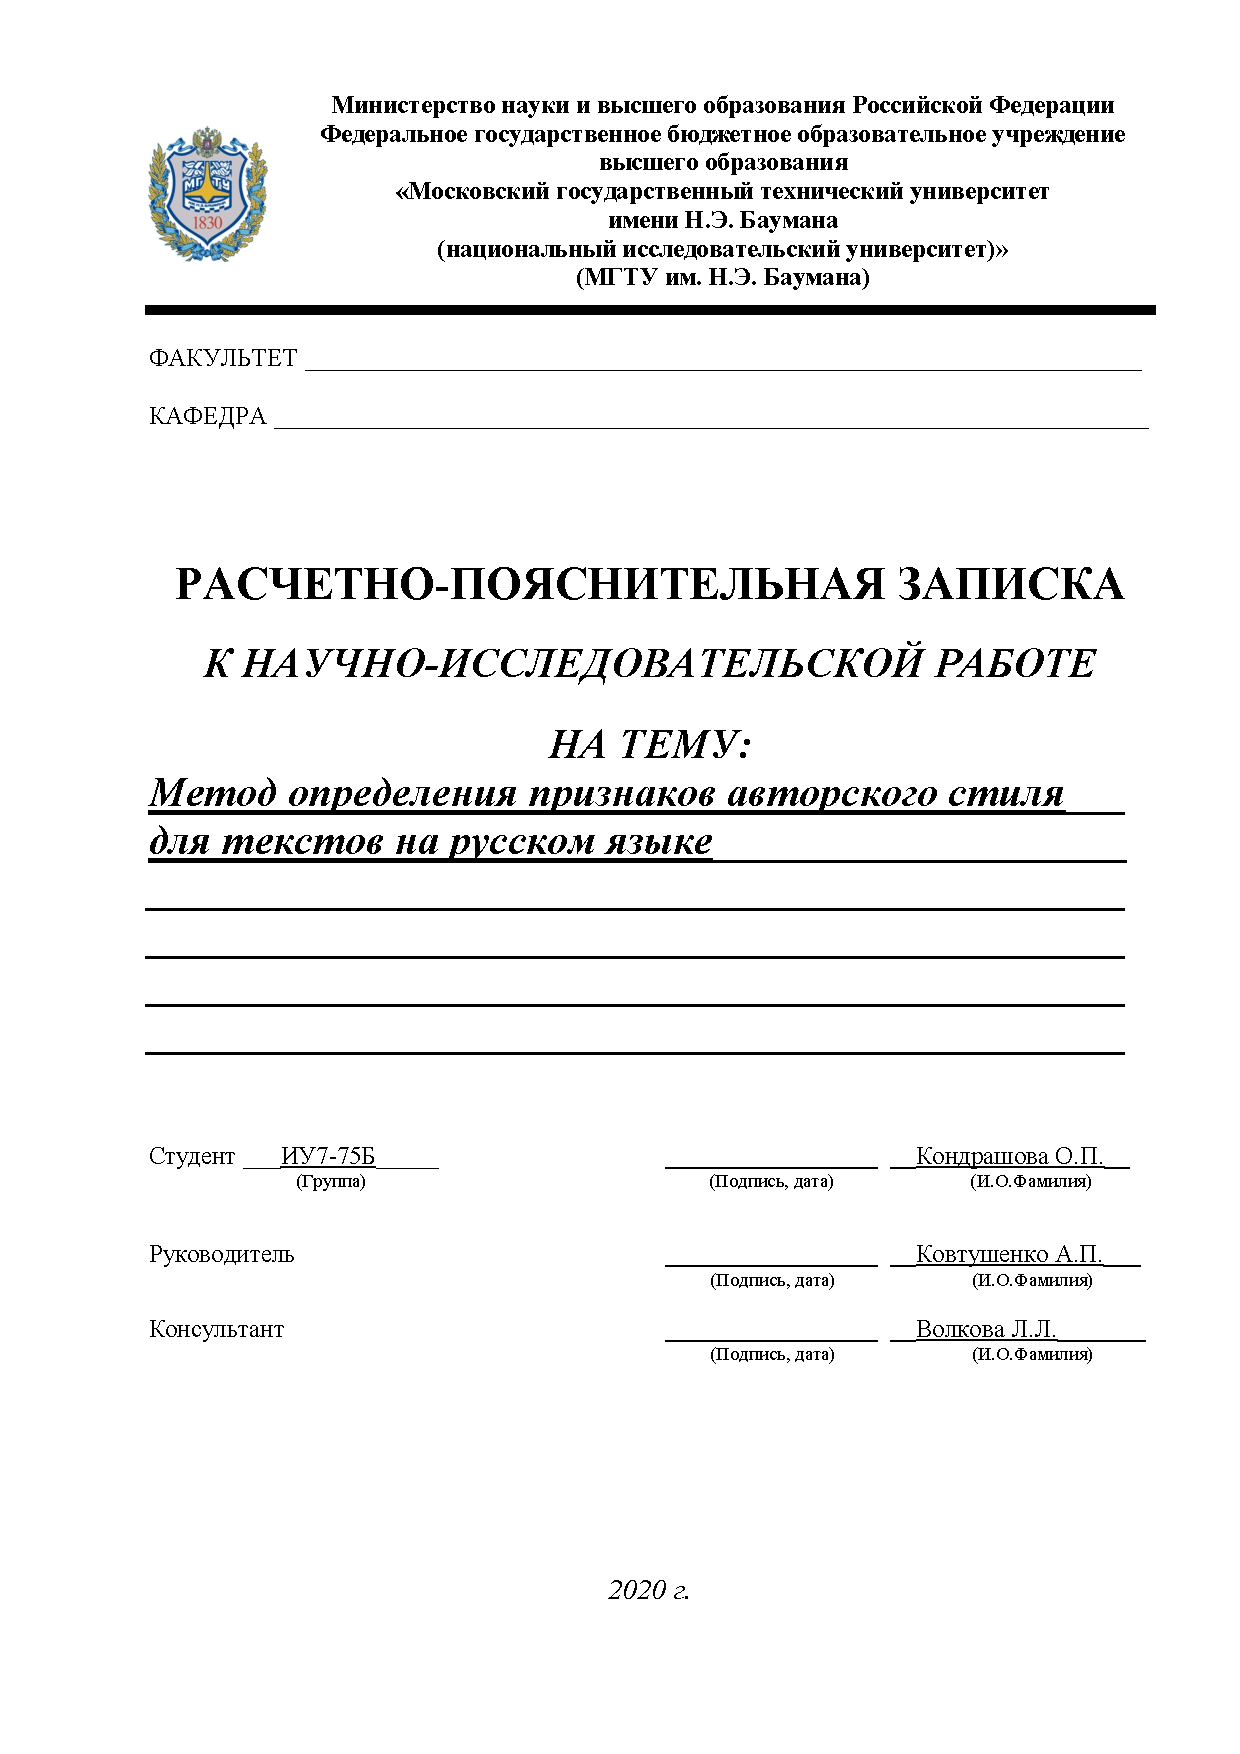
\includepdf[pages=-]{pages/title.pdf}
% пропущены страницы под тз и план (у меня их 2 тз и 1 план, итого 3, вам надо пропустить столько, сколько страниц у вас в тз и плане)


%\listoffigures                         % Список рисунков

%\listoftables                          % Список таблиц

%\NormRefs % Нормативные ссылки 
% Команды \breakingbeforechapters и \nonbreakingbeforechapters
% управляют разрывом страницы перед главами.
% По-умолчанию страница разрывается.

% \nobreakingbeforechapters
% \breakingbeforechapters

\tableofcontents

% \printnomenclature % Автоматический список сокращений

\include{12-intro}

\mainmatter % это включает нумерацию глав и секций в документе ниже

\include{20-analytical}
\include{30-design}
%\include{50-research}

\backmatter %% Здесь заканчивается нумерованная часть документа и начинаются ссылки и
            
\include{80-conclusion}%% заключение

\begin{thebibliography}{}
\bibitem{stylometry} Мартыненко Г. Я. (2015). Стилеметрия: Возникновение и становление в контексте междисциплинарного взаимодействия. Часть 2. Первая половина XX в.: Расширение междисциплинарных контактов стилеметрии. СТРУКТУРНАЯ И ПРИКЛАДНАЯ ЛИНГВИСТИКА, (11), 9-28.
\bibitem{invariant} Фоменко В.П., Фоменко Т.Г. Авторский инвариант русских литературных текстов. Предисловие А.Т. Фоменко // Фоменко А.Т. Новая хронология Греции: Античность в средневековье. Т. 2. М.: Изд-во МГУ, 1996. С.7 68-820.
\bibitem{tokenization} Ермакович М.В. Автоматическое определение границ слова в русском тексте с помощью комплекса лингвистических правил. Компьютерная лингвистика и интеллектуальные технологии: по материалам международной конференции «Диалог 2017» Москва, 31 мая — 3 июня 2017.
\bibitem{tutorial} Автоматическая обработка текстов на естественном языке и компьютерная лингвистика: учеб. пособие / Большакова Е.И., Клышинский Э.С., Ландэ Д.В., Носков А.А., Пескова О.В., Ягунова Е.В.
\bibitem{synt} Шелманов А.О., Исследование методов автоматического анализа текстов и разработка интегрированной системы семантико-синтаксического анализа.
\bibitem{chomsky} Chomsky N. Three models for the description of language // IRE Transactions on Information Theory. — 1956. — Vol. 2, no. 3. — P. 113–124.
\bibitem{tesniere} Tesnière L. Elements de syntaxe structurale. — Editions Klincksieck, 1959.
\bibitem{melcuk} Mel’cuk I. A. Dependency syntax: theory and practice. — ŠUNY Press, 1988. — P. 428.
\bibitem{entropy1} Хмелев Д.В. Классификация и разметка текстов с использованием методов сжатия данных [электронный ресурс] - режим доступа: URL: http://compres­sion.ru/download/articles/classif/intro.html (дата обращения: 14.03.2021).
\bibitem{batura} Батура Т. В. Формальные методы установления авторства текстов и их реализация в программных продуктах // Программные продукты и системы. 2013. №4. 
\bibitem{analyzator} Шевелев О. Г. Методы автоматической классификации текстов на естественном языке : учебное пособие / О. Г. Шевелев ; науч. ред. В. В. Поддубный ; Том. гос. ун-т. - Томск : ТМЛ-Пресс, 2007. 
\bibitem{avtoroved} Романов А.С., Мещеряков Р.В. Компьютерная лингвистика и интеллектуальные технологии: По материалам ежегодной Международной конференции «Диалог»(Бекасово, 26-30 мая 2010 г.). М.: Изд-во РГГУ
\bibitem{hoodlomer} Программы анализа и лингвистической обработки текстов. Русская виртуальная библиотека [электронный ресурс] - режим доступа: URL: https://rvb.ru/soft/catalogue/c01.html (дата обращения: 20.12.2020).
\bibitem{ngrams} Гудков В. Ю., Гудкова Е. Ф. N-граммы в лингвистике // Вестник Челябинского государственного университета. 2011. № 24 (239). Филология. Искусствоведение. Вып. 57. С. 69–71.
\bibitem{skipgrams} Guthrie David, Allison Ben, Liu Wei, Guthrie Louise, Wilks Yorick. (2006). A Closer Look at Skip-gram Modelling. Proc. of the Fifth International Conference on Language Resources and Evaluation. 
\end{thebibliography}

\end{document}

%%% Local Variables:
%%% mode: latex
%%% TeX-master: t
%%% End:
